\documentclass[12pt]{scrartcl}

% sonderzeichen encoding
\usepackage[utf8]{inputenc}
\usepackage[T1]{fontenc}
\usepackage[ngerman]{babel}

% alternating rowcolors in tables
\usepackage[table]{xcolor}
\rowcolors{2}{blue!15}{white}

% bilder
\usepackage{graphicx}

% pdf includes
\usepackage{pdfpages}

% toc als links gerendert
\usepackage[hidelinks]{hyperref}

% images in header & footer
\usepackage{fancyhdr}
\pagestyle{fancy}
\rhead{
\includegraphics[width=2cm]{images/gns}}

%listing (source code)
\usepackage{listings}
\lstdefinelanguage{JavaScript}{
  keywords={typeof, new, true, false, catch, function, return, null, catch, switch, var, if, in, while, do, else, case, break},
  keywordstyle=\color{blue}\bfseries,
  ndkeywords={class, export, boolean, throw, implements, import, this},
  ndkeywordstyle=\color{darkgray}\bfseries,
  identifierstyle=\color{black},
  sensitive=false,
  comment=[l]{//},
  morecomment=[s]{/*}{*/},
  commentstyle=\color{purple}\ttfamily,
  stringstyle=\color{red}\ttfamily,
  morestring=[b]',
  morestring=[b]"
}

\lstset{
   language=JavaScript,
   backgroundcolor=\color{lightgray!50},
   extendedchars=true,
   basicstyle=\footnotesize\ttfamily,
   showstringspaces=false,
   showspaces=false,
   numbers=left,
   numberstyle=\footnotesize,
   numbersep=9pt,
   tabsize=2,
   breaklines=true,
   showtabs=false,
   captionpos=b
}

% show lof and lot in toc
\usepackage[nottoc]{tocbibind}

% appendix package
\usepackage[toc,page]{appendix}

% deutscher appendix name
\addto\captionsngerman{\let\appendixtocname\appendixname%
\let\appendixpagename\appendixname}




\titlehead{\centering
\includegraphics[width=6cm]{images/gns}}
\title{
	Projektbericht: Erstellung einer Webanwendung
	zur Verbesserung des Workflows des Erstellens von Benutzerhandbüchern
}
\author{
	Oliver Herrmann \\
	Geb.: 23.09.1992 \\
	GNS mbH \\
	Tel.: ---- \\
	Email: oliver.herrman@gns.de \\
	Ausbildungsberuf: Fachinformatiker Anwendungsentwicklung \\
	\\
	GNS mbH \\
	Frohnhauser Str. 67 \\
	45127 Essen
}
\date{\today, Essen}

\begin{document}


%\maketitle
\thispagestyle{empty}

\begin{center}
	\huge \bfseries
		Projektbericht: Erstellung einer Webanwendung
		zur Verbesserung des Workflows des Erstellens von Benutzerhandbüchern \\[4cm]

	\Large	\mdseries

	\textbf{Auszubildender} \\
	Oliver Herrmann \\
	Geb.: 23.09.1992 \\
	GNS mbH \\
	Tel.: +49 201 109 - 1523 \\
	Email: \href{mailto:oliver.herrmann@gns.de}{oliver.herrmann@gns.de}  \\
	Ausbildungsberuf: Fachinformatiker Anwendungsentwicklung \\[2cm]

	\textbf{Ausbildungsbetrieb} \\
	GNS mbH \\
	Frohnhauser Str. 67 \\
	45127 Essen \\[3cm]

	\today, Essen
\end{center}


\newpage

\tableofcontents
\newpage



\section{Einleitende Worte}
\label{sec:einleitende-worte}
...
blondgelockter Knabe mit kohlrabenschwarzem Haar auf die grüne Bank
sich setzte, die gelb angestrichen war.


Alice kann es einfach nicht lassen, sie muß dem weißen Kaninchen mit
der großen Uhr folgen und landet prompt im Wunderland. Auf ihrer Reise
durch diese fröhlich bunte, aber auch sehr eigenartige Welt begegnet
sie einer gestiefelten Raupe, dem verrückten Hutmacher und ist zu Gast
bei einer nicht Geburtstags-Party. Einer hinterlistigen Tigerkatze hat
es das Mädchen schließlich zu verdanken, daß sie den Zorn der
Herz-Königin auf sich zieht. So etwas kann einem eigentlich nur im
Traum passieren.


\subsection{Test}

\begin{itemize}
  \item Alice im Wunderland
  \item Till Eulenspiegel
  \item Harry Potter
  \begin{itemize}
    \item Der Stein der Weisen
    \item Kammer des Schreckens
    \item Der Gefangene von Askaban
    \item Der Feuerkelch
    \item Der Orden des Phönix
  \end{itemize}
  \item Jim Knopf
\end{itemize}

zurück zu Abschnitt \ref{sec:einleitende-worte}

\subsection{IDE}

In Abbildung \ref{fig:eclipse-ide} ist eclipse zu sehen.

\begin{figure}[!ht]
	\centering
	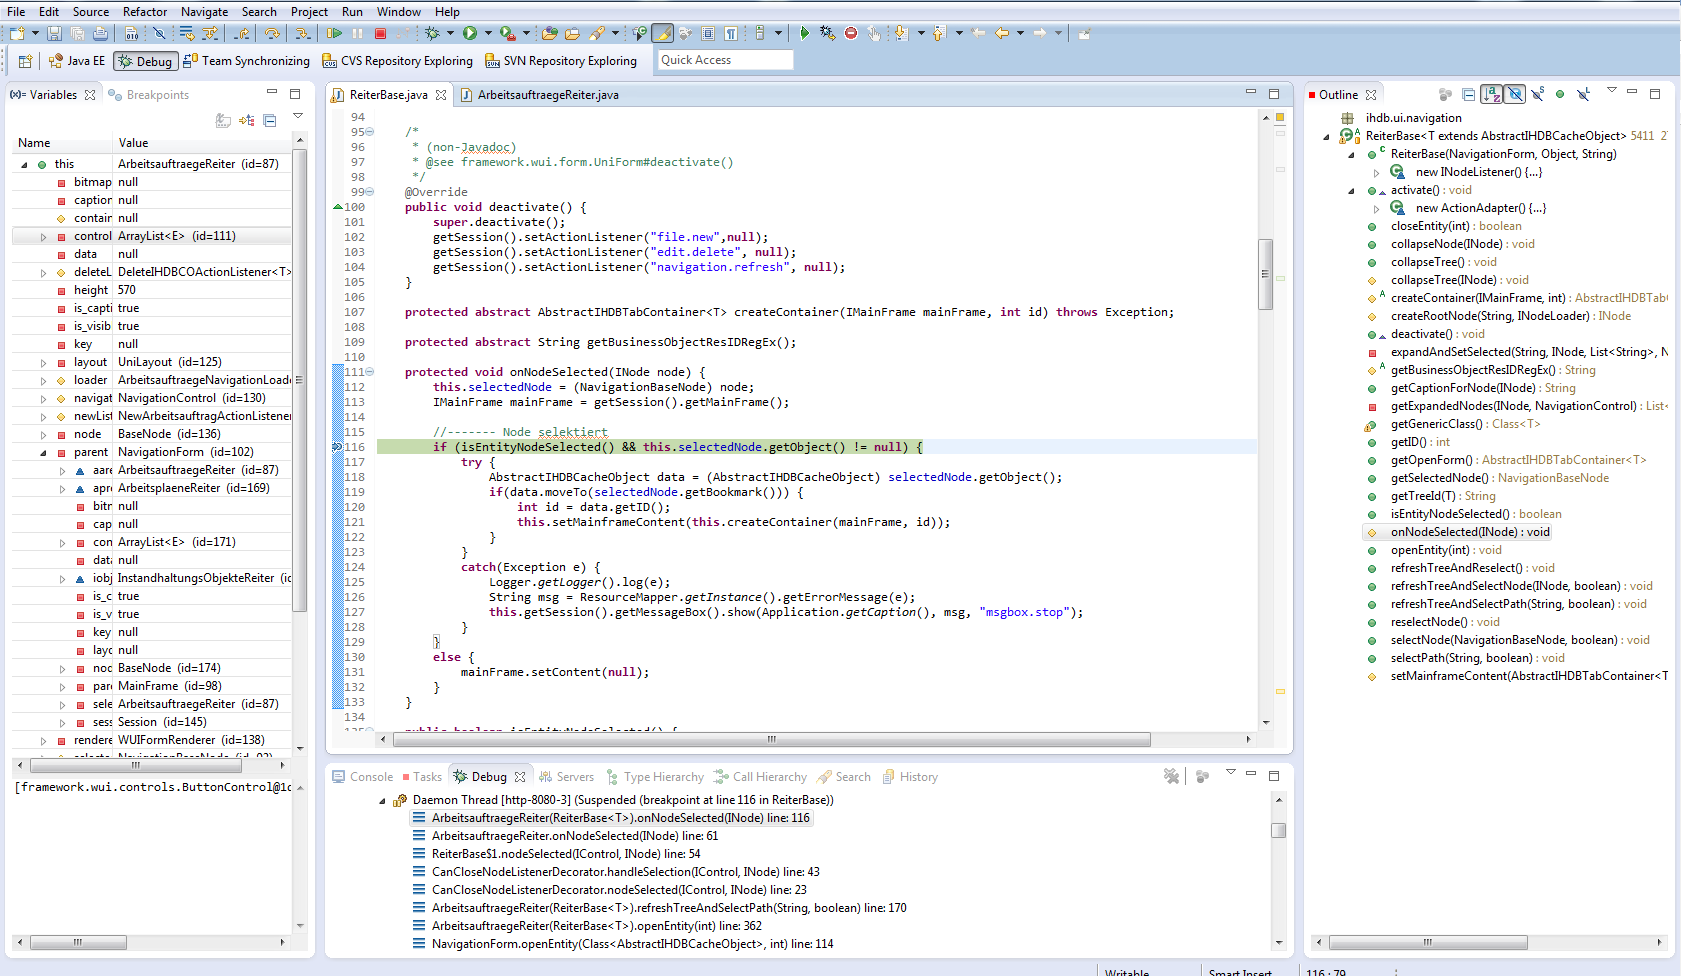
\includegraphics[width=0.8\textwidth]{images/eclipse1}	
	\caption{Eclipse IDE}
	\label{fig:eclipse-ide}
\end{figure}



\subsection{test2}

\begin{enumerate}
	\item erstens
	\item zweitens
\end{enumerate}


\section{Tables}

	Siehe \hyperref[tab:test]{Beispieltabelle}

	\begin{table}
	\centering
	\begin{tabular}{c|c}

		\rowcolor{gray!15}
	    Table head & Table head \\\hline

	    Some values & Some values \\\hline
    
	    Some values & Some values \\\hline
	    
	    Some values & Some values
	    

	\end{tabular}
	\caption{Testdaten}
	\label{tab:test}
	\end{table}

\clearpage

\begin{appendices}
\renewcommand{\thesection}{\arabic{section}} %\Roman{section}

\addtocontents{toc}{\protect\setcounter{tocdepth}{1}}

	\section{First appendix}		
		\subsection{First app. subsection 1}
		Lorem ipsum...

	\newpage
	\section{Rechtschreibfehler}
		\begin{center}
			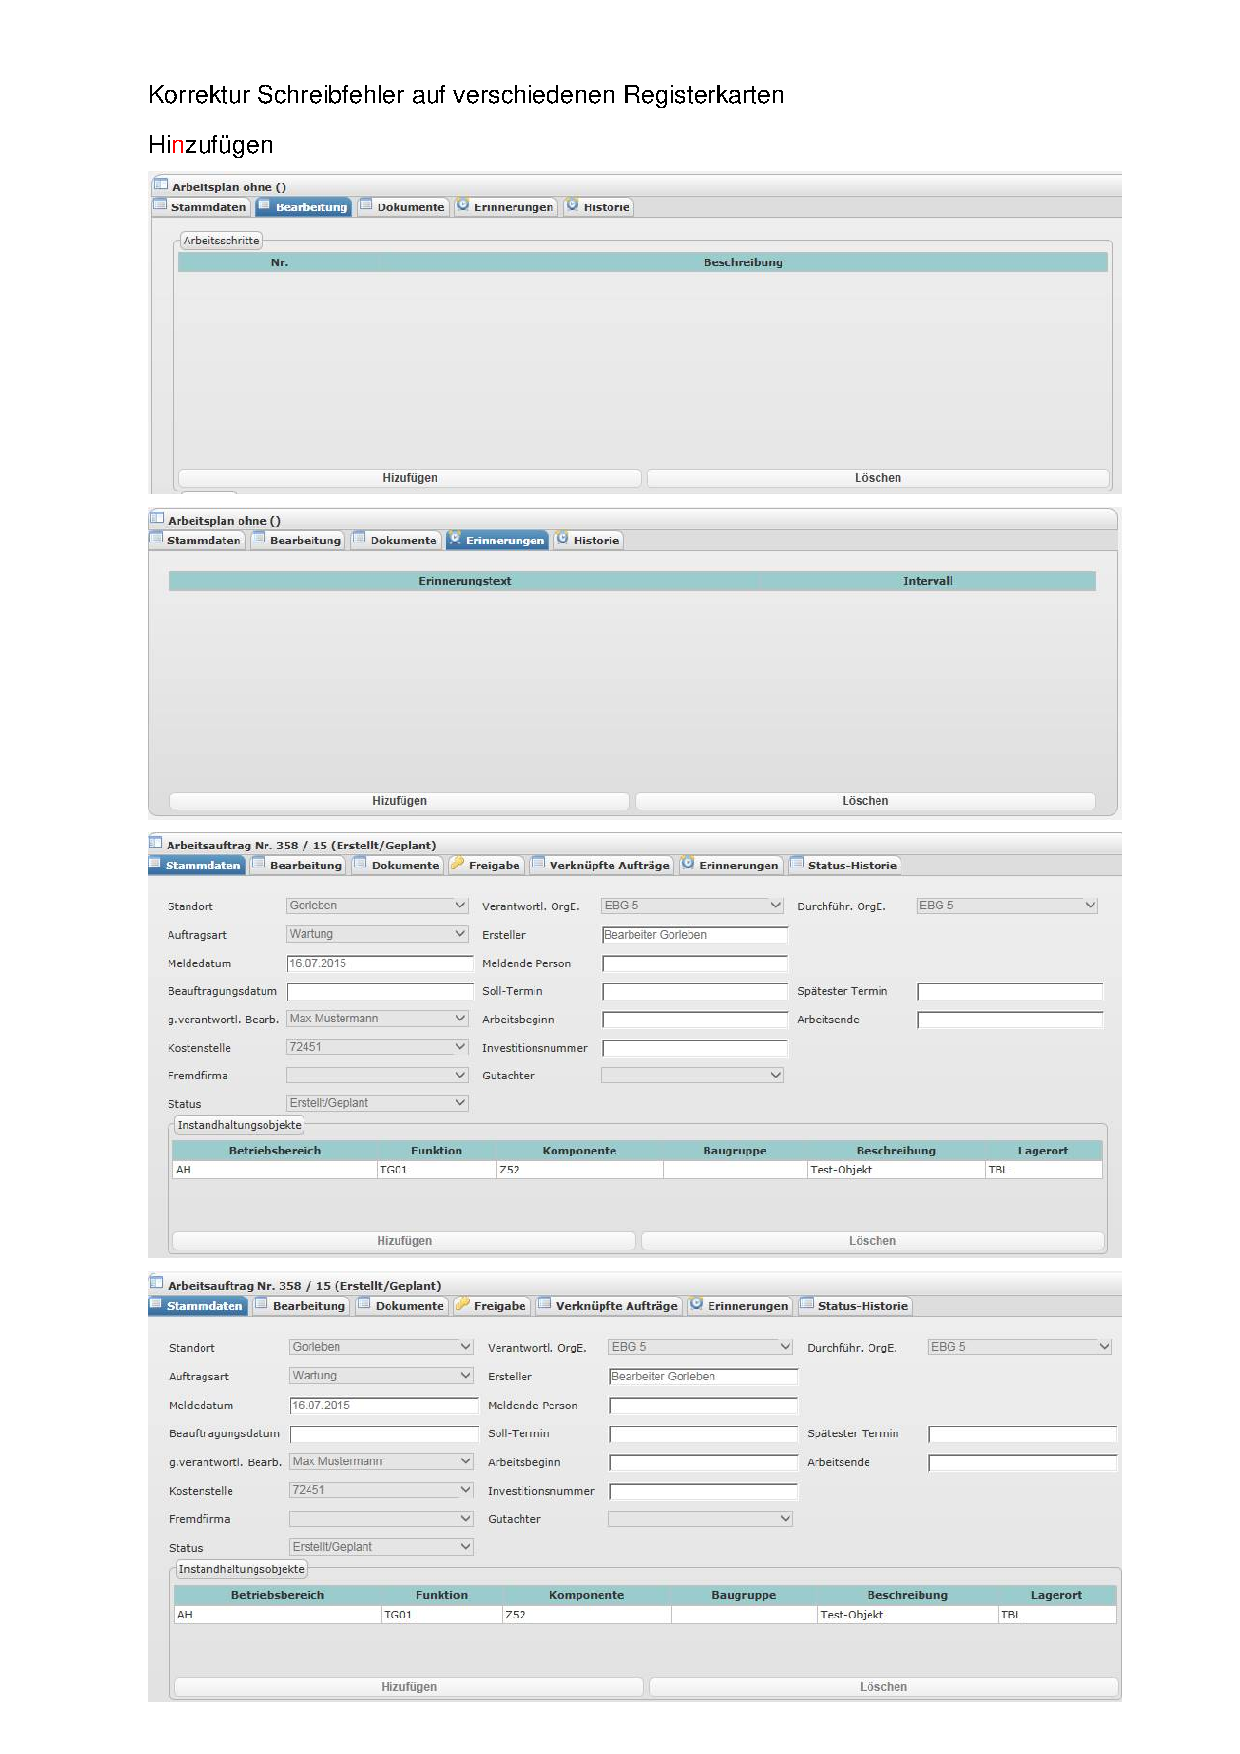
\includegraphics[page=1, width=.85\textwidth]{pdf/test.pdf}		
		\end{center}

	\newpage		
	\section{Pflichtenehft}
		\inputencoding{utf8}

\subsection*{Zielbestimmung}

	\subsubsection*{Musskriterien}
		\begin{itemize}
			\item Benutzerverwaltung
			\begin{itemize}
				\item Benutzer anlegen
				\item Benutzerdaten editieren
				\item Benutzer löschen
			\end{itemize}
			\item Wikiverwaltung
			\begin{itemize}
				\item Wiki anlegen
				\item Wikidaten editieren
				\item Wiki löschen
				\item Handbuch aus Wiki generieren
				\item Handbuch runterladen
			\end{itemize}
		\end{itemize}

	\subsubsection*{Wunschkriterien}
		\begin{itemize}
			\item Handbuchversionen
			\begin{itemize}
				\item Handbuchhistorie eines Wikis einsehen
				\item Handbuch aus Historie löschen
				\item älteres Handbuch runterladen
			\end{itemize}
			\item Handbuchgenerierung
			\begin{itemize}
				\item Aktuellen Fortschritt während Generierung anzeigen
				\item Erstellung für Wikis sperren, während aktuelle Generierung läuft
			\end{itemize}
			\item Gruppenverwaltung
			\begin{itemize}
				\item Gruppen anlegen
				\item Gruppen löschen
				\item Benutzer Gruppen zuteilen
				\item Rechte Gruppen zuteilen
			\end{itemize}
		\end{itemize}

	\subsubsection*{Abgrenzungskriterien}
		\begin{itemize}
			\item Single-Sign-On über GNS internes ActiveDirectory
			\item Anlegen / Konfigurieren der Laufumgebung innerhalb der GNS DMZ
		\end{itemize}

\subsection*{Produkteinsatz}

	\subsubsection*{Anwendungsbereiche}
		Technischer/administrativer Anwendungsbereich.

	\subsubsection*{Zielgruppen}
		Die Zielgruppe besteht ausschließlich aus Mitarbeitern der GNS mbH.
		Vornehmlich wird das Produkt durch Angestellte der Abteilung
		KIS\footnote{Abteilung für softwareentwicklung} benutzt werden.

	\subsubsection*{Betriebsbedingungen}
		Das Produkt wird als Webanwendung bereitgestellt. Das Produkt ist über das Internet erreichbar.
		Es wird eine Up-Time von nahezu 100\% angestrebt.


\subsection*{Produktübersicht}
	Das Produkt ist eine Webapplikation, welche es dem Benutzer erlaubt den Inhalt eines existierenden
	Mediawikis in eine PDF- respektive HTML-Datei zu konvertieren und diese anschließend herunterzuladen.
	Hierzu kann der Nutzer selbstständig neue Wikis indizieren um diese für das spätere Konvertieren
	bereitzustellen. Konvertierte Mediawikis können anderen Benutzern ebenfalls zum download bereitgestellt
	werden.

\subsection*{Produktfunktion}
	\textbf{/F10/} \\
	\textbf{Anwendungsfall:} Handbuch generieren \\
	\textbf{Ziel:} neues Handbuch (PDF- und HTML-Dateien) aus einem Wiki generieren \\
	\textbf{Kategorie:} primär \\
	\textbf{Vorbedingung:}
		\begin{itemize}
			\item Benutzer ist eingeloggt
			\item Wiki ist registriert
			\item Benutzer ist berechtigt aus dem Wiki ein Handbuch zu generieren
		\end{itemize}
	\textbf{Nachbedingung Erfolgt:} Das neue Handbuch wird in der Historie angezeigt. \\
	\textbf{Nachbedingung Fehlschlag:} Dem Benutzer wird eine Fehlermeldung angezeigt. \\
	\textbf{Auslösendes Ereignis:} Der Benutzer startet die Generierung über einen Button. \\
	\textbf{Beschreibung:}
		\begin{enumerate}
			\item Der Benutzer klickt auf den Button \textit{Handbuch generieren}
			\item Die Handbuchgenerierung wird serverseitig durchgeführt.
			\item Die Anwendung teilt dem Benutzer in regelmäßigen Abständen den Fortschritt der Generierung mit
			\item Das fertig generierte Handbuch wird in der Handbuchhistorie des Wikis gelistet
		\end{enumerate}
	\textbf{Erweiterungen:}
		\begin{enumerate}
			\item nach der erfolgreichen Generierung wird der Benutzer gefragt, ob er das Handbuch direkt runterladen möchte
		\end{enumerate}
	\textbf{Alternativen:} -



\subsection*{Produktdaten}
	Die vom Produkt persisten gespeicherten Daten sind im Abschnitt Datenmodell beschrieben.

\subsection*{Produktleistungen}
	\textbf{/L10/}
		Während der Generierung eines Handbuchs aus einem Wiki ist dieses Wiki für alle Benutzer gesperrt, um so serverseitige Fehler bei der Generierung zu minimieren.


\subsection*{Qualitätsanforderungen}
	\begin{table}[!ht]
		\centering
		\begin{tabular}{l|c|c|c|c}
			\rowcolor{gray!15}
			\textbf{Qualitätsmerkmal}	& \textbf{sehr gut}	& \textbf{gut}	& \textbf{normal}	& \textbf{nicht relevant}	\\
			\textit{Funktionalität} 	&					&				&					&							\\
			Angemessenheit				&					&				& X					&

		\end{tabular}
	\end{table}

\subsection*{Benutzeroberfläche}
	Die Benutzeroberfläche orientiert sich an den Anforderungen von Material Design
	\footnote{\url{https://www.google.com/design/spec/material-design/introduction.html}}.
	Das Farbschema orientiert sich am Corporate Design der GNS.


\subsection*{Nichtfunktionale Anforderungen}
	Das Produkt gewährleistet die Einhaltung lokaler Gesetze bezüüglich des Datenschutzes personenbezogener Daten.

\subsection*{Technische Produktumgebung}

	Das Produkt wird final in der DMZ-Umgebung der GNS betrieben werden.

	\subsubsection*{Software}
		Das Produkt wird mithilfe eines Tomcat ServletContainers der Version 6 oder neuer betrieben.

	\subsubsection*{Hardware}

	\subsubsection*{Orgware}

	\subsubsection*{Produktschnittstellen}

		
	\newpage
	\section{Quellcode (Auszüge)}
		\lstinputlisting[language=JavaScript, caption=Test.js]{code/test.js}


\end{appendices}

\clearpage
\listoffigures
\newpage

\listoftables
\newpage

\end{document}